\documentclass[english,course]{Notes}

\title{Large Cardinals}
%\subject{SUBJECT}
\author{Amelia Harrison}
\email{amelia.j.harrison@gmail.com}
\speaker{Josh Dever}
\date{16}{09}{2015}
\dateend{01}{12}{2015}
\place{WAG 3.16}

\begin{document}

\section{Two Notions of Size}
\lecture{16}{09}{15}

We consider two notions of size: 
\begin{enumerate}
\item[(i)] $a \leq b$ iff $a$ comes before $b$ in the number order (that is $a 
\in b$), and
\item[(ii)] $a \leq b$ iff there exists an injection from $a$ to $b$. 
\end{enumerate}
This distinction is noted in language. We use words like ``one,'' ``two,'' 
``three,'' to describe the former understanding, and words like ``first,'' 
``second,'' ``third,'' to describe the latter. In this lecture, we'll use these 
two notions of size to define two sets of numbers: the ordinals and the 
cardinals, corresponding to (i) and (ii) respectively. 

Note that according to (i), $\omega \leq s(\omega)$ since $\omega \in s(\omega)$. On the other hand, 
according to (ii), $s(\omega) \leq \omega$.  
Also note, that (i) is a slightly more demanding definition in that it requires  
the notion of sets and a well-ordering, while (ii) requires only the notion of 
sets.  

\begin{definition}
We say that two well-ordered sets
$\langle A, R\rangle$ and $\langle B, S\rangle$ are 
{\sl order-isomorphic} if there exists a function $f$
with domain $A$ and range $B$, such that $f$ is bijective and for every $a_1, 
a_2 \in A$, if $a_1 \leq_R a_2$ then $f(a_1) \leq_S f(a_2)$.\end{definition}

\begin{definition}
We say that a well-ordered set $X$ is {\sl downward closed} if for all $x$ in 
$X$ and for all $y$, if $y \leq x$ then $y \in X$. 
\end{definition}

\begin{remark}
If $X$ is a downward closed set of numbers then $X$ is a number. 
\end{remark}

\begin{theorem}
If $\langle A,R\rangle$ is a well-ordered set, then there exists a number to 
which it is order-isomorphic. 
\end{theorem}

\begin{proof}{(sketch)}
Let $pred(x, A, R)$ be the set of all $y$ such that $y \in A$ and $y \leq_R 
x$. 


Consider the subset of $A$ such that all its members 
are not order-isomorphic to any number. Since $A$ is well-ordered, this subset 
has a least element. Call that element $a$. Then let 
$$N = \{n: n \text{ is a number and } n \text{ is order-isomorphic to } pred(b, A, 
R) \text{ and } b \leq a\}.$$  
Note that $N$ is a downward closed set, and so by Remark 1.3 it is a number. 
Furthermore, it is easy to see that $N$ must be order-isomorphic to $a$, 
contradicting the assumption that $a$ is not order-isomorphic to any number. It 
follows that $A$ must be order-isomorphic to some number.  
\end{proof}

Theorem 1.4 tells us that every well-ordered set corresponds a to a number in 
the sense of (i). Furthermore, there is exactly one such number.
 
Now, consider the claim that every set corresponds to a number in 
the sense of (ii): 

\begin{claim} 
For every set $X$ there exists a number $n$ which bijects 
with $X$. 
\end{claim}

It turns out that we can neither prove nor disprove this claim on the 
basis of the axioms introduced so far---it is independent. To resolve 
the claim affirmatively, we introduce the following axiom. 

\medskip

\noindent {\sc axiom of choice.} 
{\sl For every set $X$ there exists a relation $R$ such that
$\langle X, R\rangle$ is a well-ordered set.}

\medskip

Notice that this axiom makes a very tall claim. We haven't yet seen how to define the real 
numbers, but we will see that soon. It's clear that the natural ordering on the 
reals is not a well-ordering. (In fact, density defeats well-ordering on sets 
with more than one element.) [Definition of density?] 
Although it's not obvious how we can well-order 
the real numbers, the axiom of choice tells us that there is a way. In fact, 
given the axiom of choice, we can derive some pretty counterintuitive results (e.g. 
Banach-Tarski paradox). But we need it, if we want to be able to assign a 
cardinality to any set. So it's a ``pick-your-poison'' situation.   

Armed with the axiom of choice, it is easy to see how we might go about 
proving Claim 1.5: We start with a set $X$. By the axiom of choice, we know 
there exists a well-ordered set of the form $\langle X, R \rangle$. Then by 
Theorem 1.4 there is some number $n$ which is order-isomorphic to $\langle X, R 
\rangle$. Then $n$ bijects with $\langle X, R \rangle$ and therefore it must 
biject with $X$. So we found a number $n$ which bijects with $X$. But there's one 
an issue to be dealt with. We have found a number $n$ that bijects with $X$, but there's no reason to 
believe that $n$ is unique. In general there may be many well-orderings on $X$ 
and they need not order-biject. See Figure 1. 
Furthermore, we've already established that if $X$ bijects with $\omega$, for 
example, then it must also biject with $s(\omega)$.   

\medskip

%\begin{center}
\begin{figure}
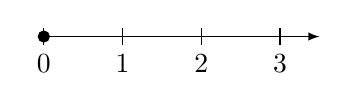
\begin{tikzpicture}
\draw[-latex] (0,0) -- (3.5,0);
\path [draw=black, fill=black] (0,0) circle (2pt);
\foreach \x in  {0,1,2,3}
\draw[shift={(\x,0)},color=black] (0pt,3pt) -- (0pt,-3pt);
\foreach \x in {0,1,2,3}
\draw[shift={(\x,0)},color=black] (0pt,0pt) -- (0pt,-3pt) node[below] 
{$\x$};
\end{tikzpicture}
%\end{center}
%\begin{center}
\hspace{2cm}
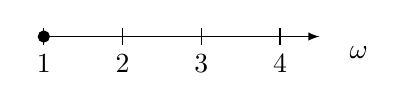
\begin{tikzpicture}
\draw[-latex] (1,0) -- (4.5,0);
\path [draw=black, fill=black] (1,0) circle (2pt);
\foreach \x in  {1,2,3,4}
\draw[shift={(\x,0)},color=black] (0pt,3pt) -- (0pt,-3pt);
\foreach \x in {1,2,3,4}
\draw[shift={(\x,0)},color=black] (0pt,0pt) -- (0pt,-3pt) node[below] 
{$\x$};
\draw[shift={(5,0)},black=white] (0pt,0pt) -- (0pt,0pt) node[below] {$\omega$}; 
\end{tikzpicture}
\caption{These two well-orderings on the natural numbers  
are not order-isomorphic. The well-ordered 
set on the left is order-isomorphic with $\omega$, the one on the right with $s(\omega)$.} 
\end{figure}
%\end{center}

\medskip

\noindent \underline{Ordinals:} sets that are transitive and well-ordered by 
$\in$\footnote{Here, when we say ``well-ordered by $\in$'' we don't mean that 
there exists a well-ordering on these sets. In fact, no such well-ordering can 
exist, because there is no such thing as the set of all ordinals. There are, in 
some sense, too many ordinals to form a set, as we will see in the next theorem.} 

\medskip
 
\noindent \underline{Cardinals:} $x$ is a cardinal if $x$ is an ordinal, and 
there is no smaller ordinal that bijects with $x$

\begin{theorem}
There is no set containing all of the ordinals.
\end{theorem}

\begin{proof}
Suppose, for the sake of contradiction, that $ON$ is the 
set of all ordinals. Then $ON$ is also an ordinal. [Why is 
this true?] But then $ON \in ON$ which contradicts the axiom of foundation. 
\end{proof}

\begin{claim} 
For any cardinal $\kappa$ the collection of ordinals of 
size $\kappa$ is a set. 
\end{claim} 

Again we find ourselves in a position where based on the axioms we have so far, 
we are unable to resolve the claim. Consider, for example the collection of ordinals of size 
$\omega$:
$$ \omega,\;\; \omega + 1,\;\; \omega + 2,\;\; \dots.$$ 
How can we form the set of such ordinals? 
The axiom of infinity only gives us one infinite set. And comprehension, 
pairing, and union won't help us here. To resolve the claim, we need to 
introduce a new axiom. Informally, this axiom says that
if we have a set, and a function on that set, then there exists a set that is 
the image of the first set under the function. But this doesn't quite 
make sense because the definition of a function presuppposes that the the 
existence of a set representing the range. [Nice, informal explanation of what 
we mean by ``function''?] To state the axiom carefully we 
will use the language of set theory. 

\medskip

\noindent {\sc axiom of replacement.} 
$$\forall x(\forall y \in x \; \exists ! z \; \phi(y,z) \rightarrow \exists w \forall 
u \; u \in w \leftrightarrow \exists y \in x \; \phi(y, u)))$$

\medskip

Using replacement we can form a set of ordinals of the form $\omega + n$ where 
$n$ is an integer. Then we can form the ordinals $\omega * n$ 
and $\omega^n$  
where $n$ is an integer. For ordinals of any of these forms, it is fairly easy 
to see that we can use a finite tuple of integers to represent the ordinal and 
then standard diagonalization methods to show that the ordinal bijects with the 
$\omega$.  

We can also form the ordinals $\omega^\omega$ and 
$\omega^{\omega^\omega}$ and so on. Here, it is a little more difficult, but we 
can even show that these ordinals biject with $\omega$. So we have many,many 
ordinals but they all correspond to the same cardinal. Next time, we'll talk 
about how to get some new cardinals.  
\end{document}
